\chapter{INTRODUCTION}
\label{intro}

\justifying

\section{Overview}
The bulk email management system is used to send emails of magnitude in thousands and more and broadcast the message to multiple email addresses with a single operation. All the required fields such as the senders’ email addresses, subject, the html body and to addresses are selected and the sending is initiated with a button. Upon successful sending to the API endpoint the emails are processed and send through the AWS simple email services to all the users and the emails that were bounced are returned after the sending operation.It makes use of a Javascript based framework called ReactJS to input the fields and send it to the API hosted on the AWS service where an array of services are used to scale and perform the sending and retrieving of bounces.\par
\noindent
In this project, the functions to send and manage emails using serverless functions is implemented and an application is created for usability. \section{Different Kinds of Services}

The serverless functionalities utilized in this project are:

\subsection{Lambda Function}
AWS Lambda is a serverless, event-driven compute service that lets you run code for virtually any type of application or backend service without provisioning or managing servers. You can trigger Lambda from over 200 AWS services and software as a service (SaaS) applications, and only pay for what you use.\cite{awslambda}

\subsection{Simple Email Service
}

Amazon Simple Email Service (SES) is a cost-effective, flexible, and scalable email service that enables developers to send mail from within any application. You can configure Amazon SES quickly to support several email use cases, including transactional, marketing, or mass email communications. Amazon SES's flexible IP deployment and email authentication options help drive higher deliverability and protect sender reputation, while sending analytics measure the impact of each email. With Amazon SES, you can send email securely, globally, and at scale.\cite{awsses}

\subsection{Simple Notification Service}
%\begin{figure}[h]
%            \centering
%            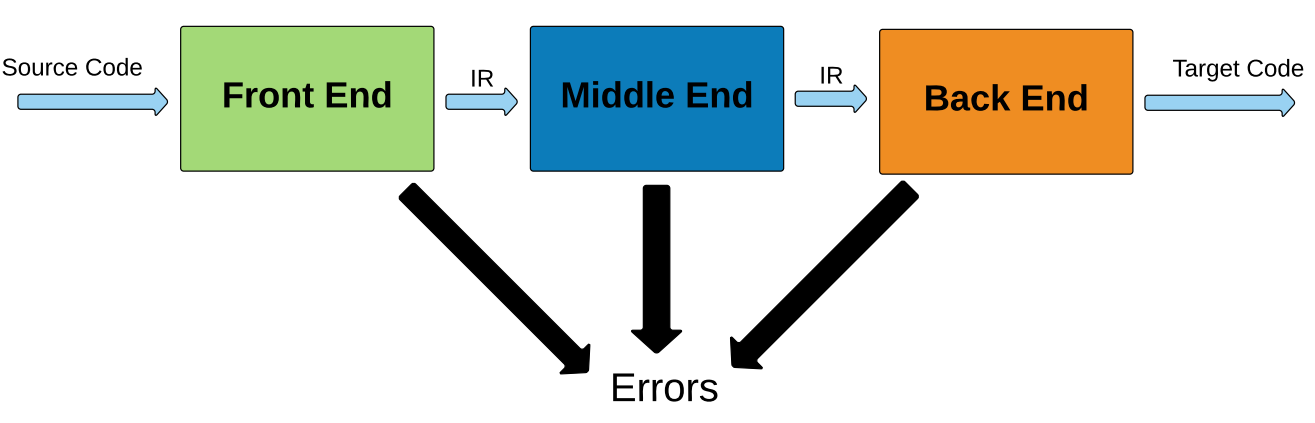
\includegraphics[width=150mm]{figures/multi_pass_compile.png}
%            \caption{Multi Pass Compiler}
%            \label{fig:multi-pass-compiler}
%\end{figure}
%
%Figure \ref{fig:multi-pass-compiler} shows a multi pass compiler which processes the source code or syntax tree of a program several times. It divides a large program into multiple small programs and processes them. It develops multiple intermediate codes. Each of the multi pass takes output of the previous pass as an input. So it requires less memory. It is also known as \textbf{Wide Compiler}. 

Amazon Simple Notification Service (Amazon SNS) is a fully managed messaging service for both application-to-application (A2A) and application-to-person (A2P) communication. The A2A pub/sub functionality provides topics for high-throughput, push-based, many-to-many messaging between distributed systems, microservices, and event-driven serverless applications. Using Amazon SNS topics, your publisher systems can fanout messages to a large number of subscriber systems, including Amazon SQS queues, AWS Lambda functions, HTTPS endpoints, and Amazon Kinesis Data Firehose, for parallel processing. The A2P functionality enables you to send messages to users at scale via SMS, mobile push, and email.\cite{awssns}
\subsection{Simple Queue Service}
Amazon Simple Queue Service (SQS) is a fully managed message queuing service that enables you to decouple and scale microservices, distributed systems, and serverless applications. SQS eliminates the complexity and overhead associated with managing and operating message-oriented middleware, and empowers developers to focus on differentiating work. Using SQS, you can send, store, and receive messages between software components at any volume, without losing messages or requiring other services to be available. 

SQS offers two types of message queues. Standard queues offer maximum throughput, best-effort ordering, and at-least-once delivery. SQS FIFO queues are designed to guarantee that messages are processed exactly once, in the exact order that they are sent. We use the FIFO queue to process the emails to be sent exactly once and make sure duplication does not occur within the list of emails.\cite{awssqs}

\subsection{API Gateway
}Amazon Application Program Interface (API) Gateway is a fully managed service that makes it easy for developers to create, publish, maintain, monitor, and secure APIs at any scale. APIs act as the "front door" for applications to access data, business logic, or functionality from your backend services. Using API Gateway, you can create Representational State Transfer (REST)ful APIs and WebSocket APIs that enable real-time two-way communication applications. API Gateway supports containerized and serverless workloads, as well as web applications.\cite{awsapi}
\subsection{CloudWatch
}Amazon CloudWatch is a monitoring and observability service built for DevOps engineers, developers, site reliability engineers (SREs), IT managers, and product owners. CloudWatch provides you with data and actionable insights to monitor your applications, respond to system-wide performance changes, and optimize resource utilization. CloudWatch collects monitoring and operational data in the form of logs, metrics, and events. You get a unified view of operational health and gain complete visibility of your AWS resources, applications, and services running on AWS and on-premises. You can use CloudWatch to detect anomalous behavior in your environments, set alarms, visualize logs and metrics side by side, take automated actions, troubleshoot issues, and discover insights to keep your applications running smoothly.\cite{awscloudwatch}
\subsection{X-ray}
AWS X-Ray helps developers analyze and debug production, distributed applications, such as those built using a microservices architecture. With X-Ray, you can understand how your application and its underlying services are performing to identify and troubleshoot the root cause of performance issues and errors. X-Ray provides an end-to-end view of requests as they travel through your application, and shows a map of your application’s underlying components. You can use X-Ray to analyze both applications in development and in production, from simple three-tier applications to complex microservices applications consisting of thousands of services.\cite{awsxray}

\newpage

\section{Problem Definition}

Given a set of emails in the form of comma separated values with their respective subjects and email content send the respective emails to everyone on the list without provisioning any form of server and track the information about the sent emails such as the bounced emails, delivered, opened and bounce rate of the from address using a dashboard.


\section{Proposed System}

The proposed system comprises of an AWS system that can serve as a serverless backend that is invoked using a REST API request made from a javascript based frontend made using the library of ReactJS.




\section{Requirements Specification}
\subsection{Software Requirements}
\begin{enumerate}
    \item Software : Any javascript enabled internet browser,Node.js 14.x .
    \item Languages : Javascript
\end{enumerate}


\subsection{Hardware Requirements}
\begin{enumerate}
    \item Random Access Memory: 2 GB.
    \item Storage: 500MB for internet browser.
\end{enumerate}
